
\section{Related Work}
Compiler-based code size reduction is important for fitting large programs to resource-constraint embedding devices. Previous approaches reduce code size by replacing a code segment with a smaller, semantically-equivalent implementation~\cite{massalin87,tanenbaum82}, deleting unnecessary code~\cite{cooper99,knoop94}, combining redundant code within a function~\cite{cocke70,chen03} or across functions~\cite{loki04,chabbi21}. Function merging falls into the later category. 

Established compilers like GCC and LLVM~\cite{llvm-fm,livska14} provide an optimization for merging identical functions at the IR level. They can only handle type mismatches that can be losslessly cast to the same format. Von~Koch~et~al.~\cite{edler14} extended this idea into merging nearly identical functions.
They restrict merging to functions with the same signature, identical control-flow graphs, corresponding basic blocks must also have the same number of instructions, and  corresponding instructions in these basic blocks must have the equivalent data type.
They only allow pairs of corresponding instructions to differ in their opcode or list of arguments.

Rocha~et~al.~\cite{rocha19} proposed a technique capable of merging arbitrary pairs of functions. They employ a sequence alignment algorithm to find equivalent code segments. These aligned functions with equivalent code can be merged into a single function. Mismatching code segments of code are also added to the merged function but have their code guarded by a function identifier. \SOAName~\cite{rocha20}, based on the sequence alignment algorithm, is the current state-of-the-art function merging technique. While promising, \SOAName still suffers from high memory usage and compilation time. As we have shown in the paper, when compiling a modest-sized program, the memory requirement of \SOAName can go well beyond what is typically available to a developer. This drawback limits the practicability and the scale at which \SOAName can operate. 
\ProjName overcomes the limitations of \SOAName with a novel alignment strategy and probability analysis. Experimental results show that our techniques significantly reduce the memory consumption and compilation time required when using the sequence alignment algorithm, allowing function merging to scale to larger programs. 


Link-time optimization can merge text-identical functions at the machine instruction level~\cite{tallam10,kwan12,msvc-icf}. This technique is hardware-specific but is orthogonal to our techniques that work at the compiler IR level. Another closely related technique is procedural abstraction~\cite{loki04,dreweke07,chabbi21}. This technique moves identical code segments to separate functions and replaces the original code segment with a function call. It requires the code texts to be fully identical,  but our function merging approach does not have this restriction. 


%\subsection{Function Merging through Sequence Alignment} \label{related:salssa}

%SalSSA~\cite{rocha20} has a search strategy for pairing similar functions for merging but avoiding a prohibitively expensive quadratic number of merging attempts.
%The purpose of the search strategy is to avoid a quadratic exploration that attempts to merge all possible pairs of functions.
%All three techniques use a ranking strategy based on the \textit{fingerprint} of the functions to evaluate their similarity.
%They start by precomputing and caching fingerprints for all functions.
%The fingerprint is a fixed-size vector that summarizes the content of the function.
%To this end, the fingerprint consists of a map of instruction opcodes to their frequency in the function.
%While functions can have several thousands of instructions, an IR usually has just a few tens of opcodes, e.g., the LLVM IR has only about 68 different opcodes.

%The fingerprint representation allows us to compare functions using a simple distance metric, such as the Manhattan distance.
%For a given reference function, all other functions are ranked based on the distance of their fingerprints.
%The candidate function with the smallest distance will be used for a merging attempt.

%By comparing the opcode frequencies of two functions, we are able to estimate
%the best case merge, which would happen if all instructions with the same opcode could match.
%This is a very optimistic estimation. It would be possible only if instruction types and order
%did not matter. We refine it further by estimating another best case merge, this time based
%on type frequencies, which would happen if all instructions with the same data type could match.

%Since the fingerprint of functions have fixed size, i.e., the number of instruction opcodes, the distance between two functions can be computed in constant time.

% \begin{figure}[h]
%   \centering
%   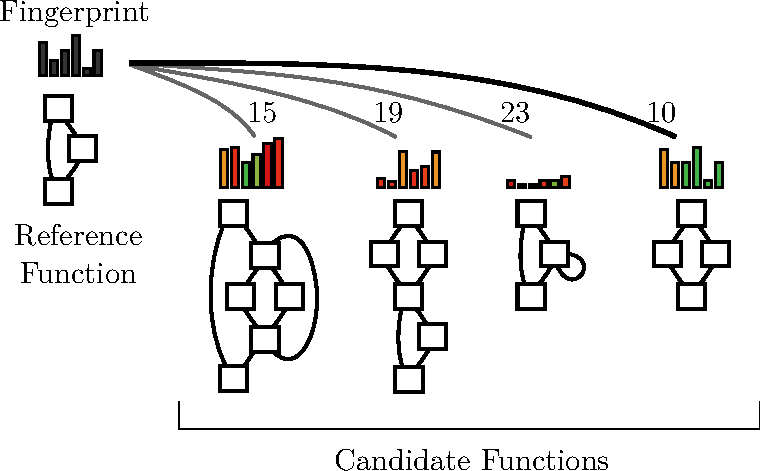
\includegraphics[width=\linewidth]{figs/hyfm-ranking.pdf}
%   \caption{.}
%   \label{fig:hyfm-ranking}
% \end{figure}

%\subsection{Merging Similar Functions}

%The function merging technique proposed by von Koch~et~al.~\cite{edler14} restricts merging to nearly identical functions.
%They only allow for pairs of corresponding instruction to differ, as long as they still have equivalent data type, where a diamond-shape branch is created to select which instruction will be executed depending on a function identifier.
%A phi-node is used to unify the mismatching instructions as a single named value.
%Every use of the mismatching instructions will refer to their phi-node.
%Two instructions match if they have the same opcode with equivalent data types and operands.
%Note that no operand selection is performed.
%Even if two instructions differ only on their operands, they are classified as mismatching, and a branch is created.

% \begin{figure}[h]
%   \centering
%   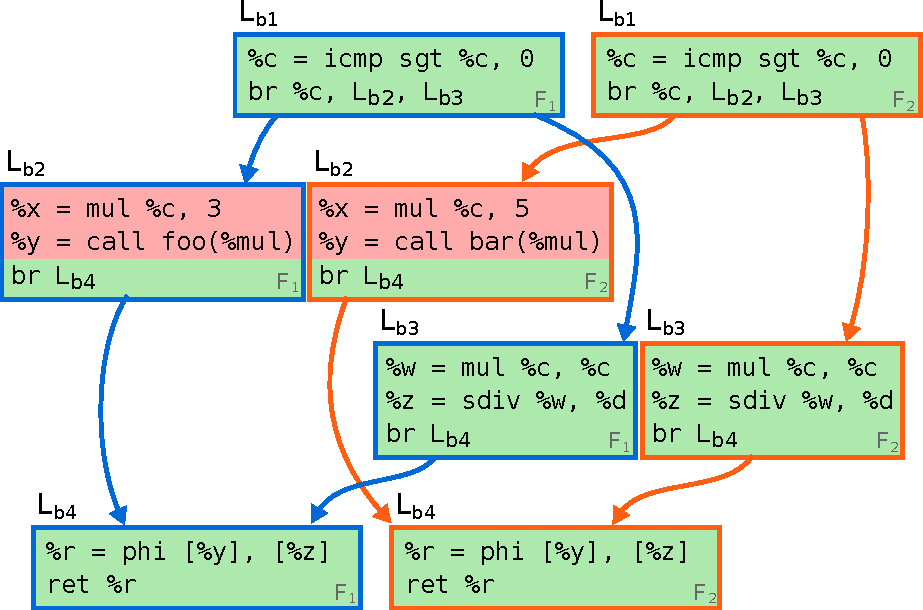
\includegraphics[width=\linewidth]{figs/soa-example-1.pdf}
%   \caption{.}
%   \label{fig:soa-example-1}
% \end{figure}

%Except for mismatching pairs of instructions, the two functions must have identical function types, i.e., they must have the same return type and list of arguments, identical CFGs, with corresponding basic blocks having the same number of instructions.

%** however, these instructions must define names representing the same data type.

% \begin{figure}[h]
%   \centering
%   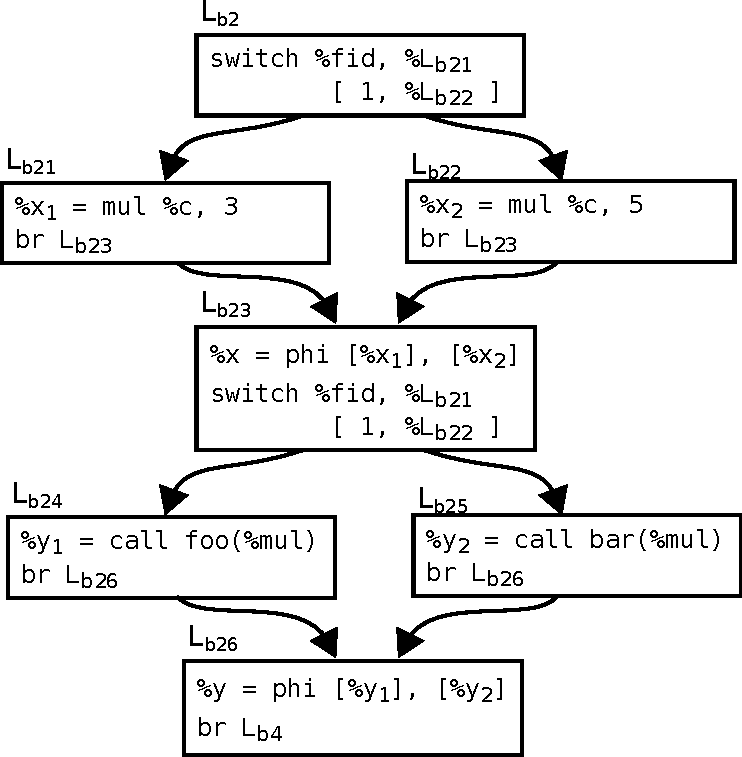
\includegraphics[width=0.8\linewidth]{figs/soa-example-2.pdf}
%   \caption{.}
%   \label{fig:soa-example-2}
% \end{figure}
